\documentclass[sigconf]{acmart}

\usepackage{booktabs} % For formal tables

% Copyright
\setcopyright{none}
%\setcopyright{acmcopyright}
%\setcopyright{acmlicensed}
%\setcopyright{rightsretained}

% DOI
%\acmDOI{10.475/123_4}

% ISBN
%\acmISBN{123-4567-24-567/08/06}

%Conference
\acmConference[PEARC17]{Practice \& Experience in Advanced Research Computing}{July 2017}{New Orleans, LO USA} 
\acmYear{2017}
\copyrightyear{2017}
\acmPrice{15.00}

\begin{document}
\title{Apache Airavata Distributed Task Execution: Designing A Flexible Framework For Managing Distributed Workload}

\author{Gourav Shenoy}
\affiliation{
  \institution{Science Gateway Research Center}
  \institution{Pervasive Technology Institute}
  \institution{Indiana University}
  \city{Bloomington} 
  \state{IN}
  \postcode{47408} }
\email{goshenoy@indiana.edu}

\author{Ajinkya Dhamnaskar}
\affiliation{
  \institution{Science Gateway Research Center}
  \institution{Pervasive Technology Institute}
 \institution{Indiana University}
  \city{Bloomington} 
  \state{IN}
   \postcode{47408}}
\email{adhamnas@iu.edu}

\author{Suresh Marru}
\affiliation{
  \institution{Science Gateway Research Center}
  \institution{Pervasive Technology Institute}
   \institution{Indiana University}
  \city{Bloomington} 
  \state{IN}
   \postcode{47408}}
\email{smarru@iu.edu}

\author{Marlon Piece}
\affiliation{
  \institution{Science Gateway Research Center}
  \institution{Pervasive Technology Institute}
   \institution{Indiana University}
  \city{Bloomington} 
  \state{IN}
   \postcode{47408}}
\email{marpierc@iu.edu}

\begin{abstract}
Managing workloads for compute-intensive and data-intensive applications is a fundamental task to provide resilient, scalable and manageable infrastructure. Scientific applications by nature are mostly compute-expensive and require high-end computational resources and may require long execution times. Based on the problems, some executions result in large datasets. Technology evolutions (occasionally disruptive) challenge the scientific application execution frameworks to adapt to paradigm changes. Cloud Computing has added on demand computing to the traditional batch queue based computing. In this paper we discuss a system design which divides workload management logic into distributed components. This design is inspired by microservice architectural principles to exploit their potential for scalability, availability, portability and, most importantly, ability to support rapid evolution. We encapsulate diverse execution patterns as Directed Acyclic Graph (DAG), thus alleviating the framework from computational paradigm changes. By capturing execution patterns as a graph, the framework itself can be generic, and the differences are encapsulated into the DAG descriptions. The DAG enactment is achieved by loosely-coupled components with well-defined communication contracts. We discuss the motivations for such a design and early validations with Apache Airavata as an implementation laboratory.   
\end{abstract}

%
% The code below should be generated by the tool at
% http://dl.acm.org/ccs.cfm
% Please copy and paste the code instead of the example below. 
%
\begin{CCSXML}
<ccs2012>
<concept>
<concept_id>10010520.10010521.10010537.10003100</concept_id>
<concept_desc>Computer systems organization~Cloud computing</concept_desc>
<concept_significance>500</concept_significance>
</concept>
<concept>
<concept_id>10002951.10003227.10010926</concept_id>
<concept_desc>Information systems~Computing platforms</concept_desc>
<concept_significance>300</concept_significance>
</concept>
<concept>
<concept_id>10011007.10011074.10011134.10003559</concept_id>
<concept_desc>Software and its engineering~Open source model</concept_desc>
<concept_significance>300</concept_significance>
</concept>
</ccs2012>
\end{CCSXML}

\ccsdesc[500]{Computer systems organization~Cloud computing}
\ccsdesc[300]{Information systems~Computing platforms}
\ccsdesc[300]{Software and its engineering~Open source model}

\keywords{Apache Airavata, Distributed Systems, Task Execution}

\maketitle

\section{Introduction}

Cyberinfrastructure is the collection of distributed computing resources, research networks, and software. Central problems in cyberinfrastructure operations involve adapting and bridging \cite{hey2005cyberinfrastructure}: we must adapt to both resource-centric views (typically adopted by computing resource providers) and scientific views of cyberinfrastructure, and we must bridge between multiple infrastructure providers. Science gateway research addresses both problems by providing web-based user interfaces and supplying services to support scientific users and communities. Science gateways by their nature provide user-centric views of infrastructure, focusing on scientific applications used by a specific field (atmospheric science, bio-informatics, computational chemistry, nanotechnology, phylogenetics, etc). Gateways also frequently need to provide access to multiple grids, local campus resources, and computing clouds to serve their communities \cite{perera2008workflow}. Gateways thus act as overlay cyberinfrastructure, federating resources that do not otherwise interoperate. Science gateway research looks for ways to encapsulate these problems within a single software framework. In this paper, we examine these requirements in greater detail, propose an architectural solution, and investigate the implementation of this solution within the Apache Airavata framework \cite{marru2011apache,marru2015apache}. 

A fundamental consideration in designing gateway architectures is that they are going to be implemented on a distributed system.  Science gateway frameworks in general, including Apache Airavata, are distributed systems.  A distributed system is an application that executes a collection of protocols to coordinate the actions of multiple processes on a network, such that all components cooperate together to perform a single or small set of related tasks. The fundamental benefit of such a system is the ability to connect remote users with remote resources in an open and scalable fashion. When we say open, we mean each component is continually open to interaction with other components. When we say scalable, we mean the system can easily be expanded to accommodate changes in the number of users, resources and computing entities. An obvious benefit of distributed systems for supercomputers is that they are powerful, but in order to be useful, they need to also be reliable.  Therefore, a fundamental goal in designing gateway architecture is to not compromise system reliability.  Airavata is a stable and reliable gateway middleware, which was a difficult goal to achieve, given the complexity of interactions between different distributed components which are running simultaneously \cite{pierce2015apache}. Our proposed design for gateway architecture is able to enhance gateway flexibility without compromising reliability.

In order to achieve reliability, a distributed system needs to be fault-tolerant, highly-available, consistent, scalable, secure and responsible \cite{burns2016design, casavant1988taxonomy}. Each of these characteristics has its own set of design challenges, and designing architectures and applications in distributed environments adds a layer of complexity to those challenges.  Below we discuss several factors that need to be considered when designing any distributed application.

\subsection{Abstraction}
Simplicity is a key ingredient for the success of any computing application; most users do not care about lower-level infrastructure details. Typically users are interested in an application's responsiveness, availability and correctness. A major challenge for any distributed system is the ability to scale dynamically, without burdening the user or compromising the usability. 

\subsection{Disruptive technologies and the opportunities}
Emerging needs and competing markets strive to come up with disruptive solutions to distributed environment problems. There are a few groundbreaking technologies like HTCondor \cite{tannenbaum2001condor,thain2005distributed}, AKKA \cite{akka}, Spark \cite{zaharia2010spark} etc., that resonate with the distributed workload management. Our solution to the problem is an amalgamation of the design inspirations from these technologies. Design decisions are heavily influenced by the nature of an application. Distributed applications are broadly classified as data-intensive and compute-intensive. Data-intensive applications devote most of their time processing large amounts of data (typically terabytes or petabytes) and processing I/O. On the other hand, compute-intensive applications demand a lot of computing power. Most of the scientific applications are compute-intensive and require supercomputers to execute jobs. Scientific applications are hard to execute on local workstations because of their high-end resource requirements. These applications run best on supercomputers or clouds.

\subsection{Heterogeneity of compute resources}
By definition, heterogeneous compute resources are hard to generalize and can be designed and configured based on business needs. HPC (High Performance Computing) and HTC (High Throughput Computing) are heavily practiced computing paradigms, and each is uniquely suited for particular types of computing problems. HPC is tailored to large computational tasks that require interactions of intermediate results to complete the computation.  HPC focuses on executing jobs that require large computing power for short duration. HTC, on the other hand, is suited to problems with large computational loads where individual computations do not need to interact while running.   HPC can be roughly termed as parallel computing on high end computing resources, and this environment is best suitable for Message Passing Interface (MPI) workloads which demand low latency and where tasks are tightly-coupled.

\subsection{Parallelism Types}
Most scientific applications consume a lot of resources and take hours to complete. In environments running these applications it is important to identify opportunities to break down larger jobs into smaller ones and then execute them simultaneously. MPI is a popular parallelization technique that makes use of available computing resources efficiently. It uses communicator objects to connect groups of processes in an MPI session. Communicator is responsible for assigning a unique identifier to a process and arranging involved processes in an ordered topology. Likewise, MapReduce is a heavily used big data framework. It splits large input datasets into multiple smaller chunks that are then processed by the Map task parallely. Output of the Map task is sorted and fed to the Reduce task. Map and Reduce tasks can be spanned across multiple nodes; this requires a special type of distributed file system known as HDFS (hadoop file system).

In summary the diversity of these parallelism patterns is exemplified by the diversity in programmed languages and their associated run time systems. These patterns  vary from simple single-threaded to multi-threaded and parallel implementations. This diversity motivates our problem to explore an architecture pattern which is easy to implement and yet facilitates evolution.   

\section{PROBLEM STATEMENT}

\subsection{Microservices-based Architecture}
Essentially, microservice architecture is a way of designing software applications as several loosely coupled, collaborating services. Each of these services implements a set of closely related functions, and can be deployed independently. Once these functions are deployed, proper design becomes critical because services in the microservice architecture have to communicate efficiently over a well defined technology-agnostic network. Communication paradigms should be lightweight, portable, and able to absorb any new changes to the application. Apache Thrift is well-suited to make  communication models portable across different languages. RabbitMQ \cite{rabbitMQ} is an elegant Advanced Message Queueing Protocol (AMQP) that gives very good control over communication channels and provides a number of helpful features. The  most critical consideration in designing a microservice-based architecture is to ensure that the system and its components are all agnostic of their surroundings; this insures that communication is not hindered by arbitrary aspects of components, such as implementation language. We accomplished this, in part, by designing with a well-defined communication infrastructure; this infrastructure helps all types of microservices communicate asynchronously.

\subsection{The Problem}
Given the complexity in designing a distributed system to support both compute- and data-intensive applications, the real challenge is to find possible solutions to the issue of managing workloads in a distributed environment. In a microservices based distributed architectures, every micro-service is responsible for performing some meaningful work. A distributed scientific application can be modelled as a sequence of executions of tasks (small units of work). The sequence depends on the type of application - compute- or data-intensive. As an example, in order to run a scientific application on an HPC cluster, we need to follow a task execution pipeline such as:

\begin{enumerate}
\item Stage the input files to the application on the target machine.
\item Setup the environment on the target machine - load necessary modules.
\item Create a job configuration file and schedule it using a resource manager.
\item Monitor the progress of the job.
\item If successful fetch the output files, or if failed report the reason for error.
\end{enumerate}

These tasks can be arranged in a workflow, or DAG (directed acyclic graph), and can be executed one by one. However,  different applications might need different DAGs; and the output may itself be a new type of task (say run analysis on the output files).  The output task needs to be added to the workflow. This leads to designing a microservices based distributed system that allows these different microservices to communicate and distribute work in a way that we ensure the following work distribution capabilities:

\begin{itemize}
\item Decoupling - the components need to be loosely coupled, such that any component or micro-service can be updated with a newer version of code without having to change or alter the other components.
\item Impedance mismatch - the communications between different components or micro-services need to follow an agreed protocol, and so does the objects used for communication. 
\item Scaling, Elasticity - as mentioned above, the design needs to be elastic and support the ability to scale individual components when necessary.
\item Fault Tolerance (Resilience) - the availability of the system should not be compromised, even in the event of a partial failure of some components. 
\item Asynchronous Communications - in a distributed system, the communications between different components are inherently asynchronous. 
\end{itemize}	

\section{PROPOSED SOLUTIONS}

\subsection{Task Execution as a Workflow}
This idea has been motivated from an understanding of the Apache Mesos \cite{apacheMesos} architecture, and how it functions. The idea is to store the task execution sequence for different application types as DAGs in a graph database. Different application types will have different DAGs. These DAGs are a codified sequence of tasks needed to perform that experiment.  Our design also includes a highly-available orchestrator component, which will centrally maintain the state of an experiment, i.e., the status of the tasks it required to complete it. The task execution DAG is determined based on the type of application being submitted via the experiment.  When the request is launched, the system will fetch the task execution DAG associated with that application and iterate through it.

\begin{figure*}
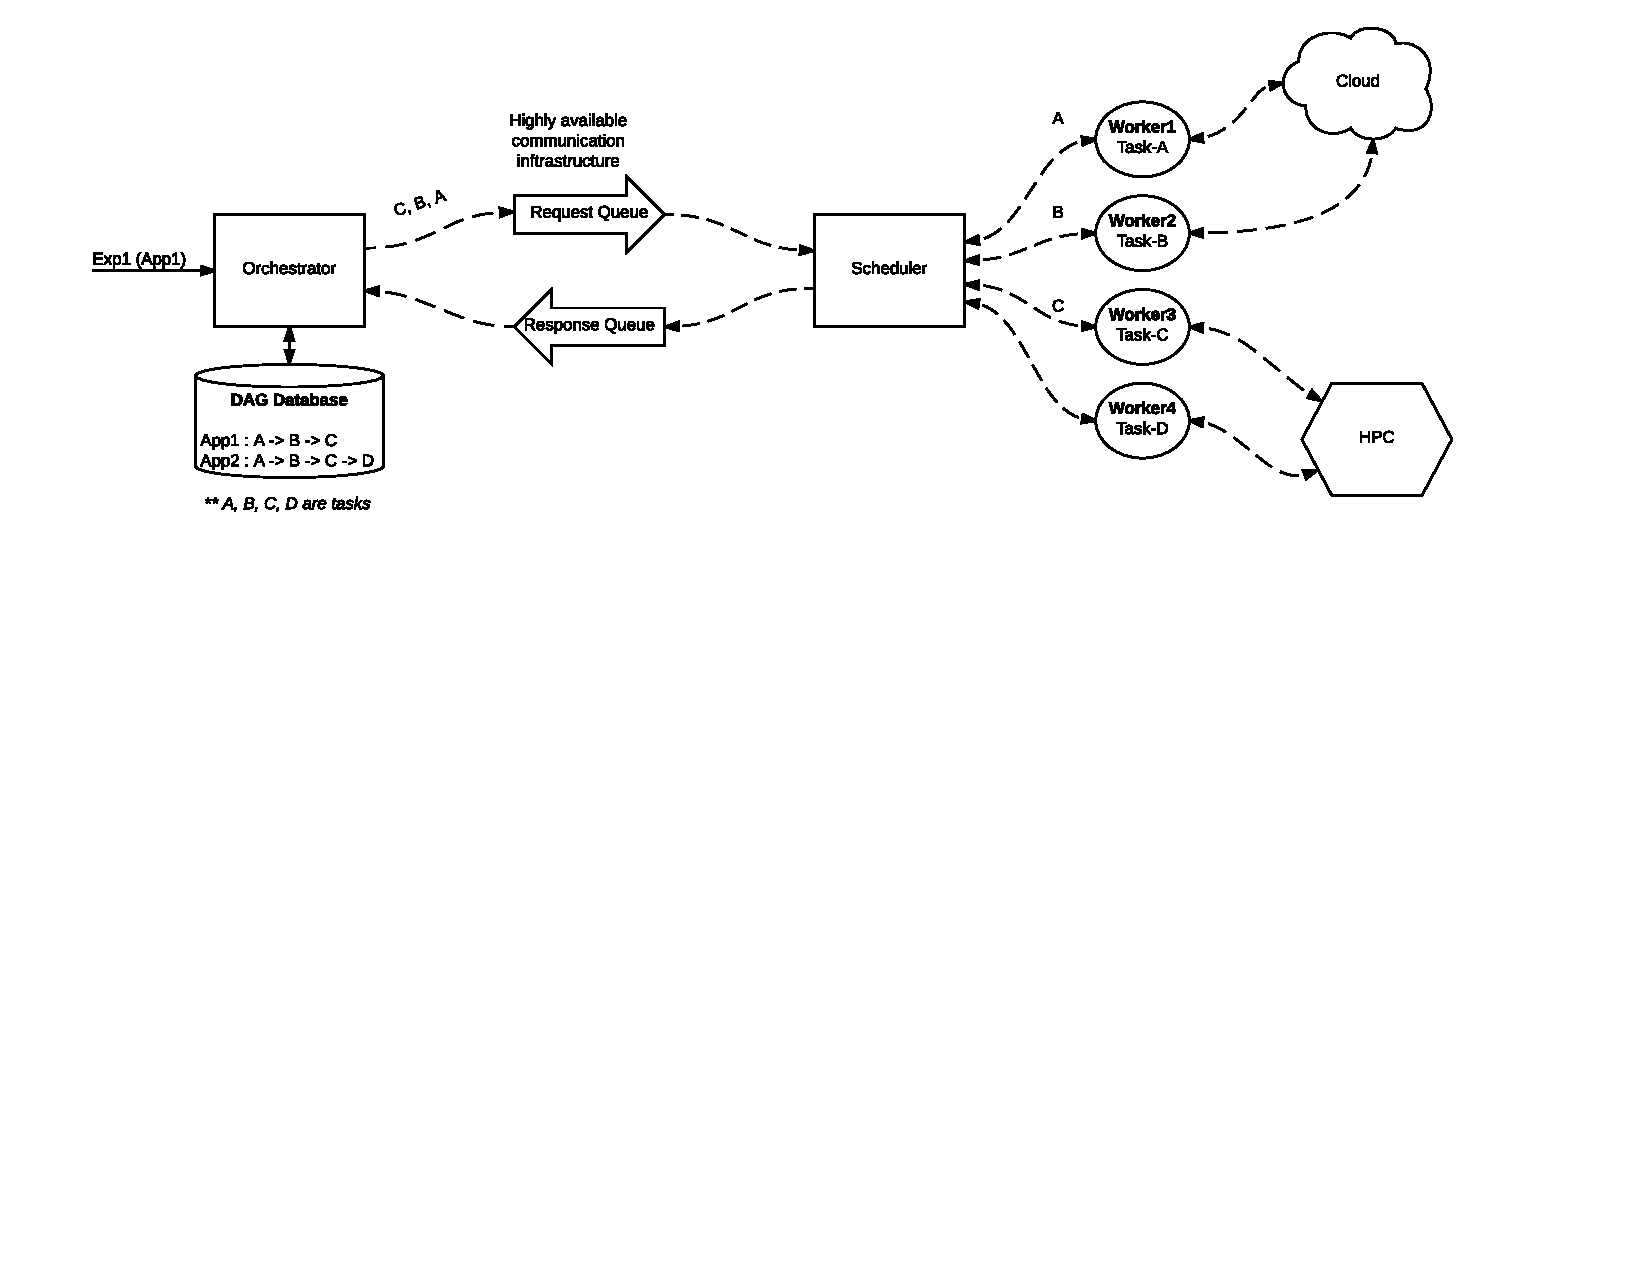
\includegraphics[height=3in, width=7in]{figures/overall-design.pdf}
\caption{Proposed Design for Distributed Task Execution.}
\end{figure*}

There is a scheduler that will receive a task execution request from the orchestrator and decide which worker to assign it to. In this context, each worker  is analogous to the current Apache Airavata GFAC module that executes the task. We can think of the worker as a collection of implementations of different tasks. E.g.,: Worker1, Worker2, Worker3, and Worker4 in the figure [x] above will have code to execute tasks A, B, C, and D respectively.

There are 2 concerns that arise here:

\begin{enumerate}
\item How does the scheduler know/decide which worker to pass the task execution to?
\item How do we upgrade a worker, say with a new task 'E' implementation, in such a manner that if something goes wrong with code for 'E', the entire worker node should not fail? In short, avoid regression testing the entire worker module.
\end{enumerate}

To address the first problem, we adopted a paradigm similar to Apache Aurora \cite{apacheAurora}.  Apache Aurora agents (workers) report available capabilities to the Aurora master (scheduler). In Aurora, the slave nodes constantly report back to the master how much processing power they have; accordingly, the master decides which slave to pass a new job request to. In our case, we can have the workers advertise to the scheduler which tasks they are capable of executing and the scheduler uses this information to make a decision as to which worker will execute a particular task.

To address the second concern, every worker node will have task implementations bundled in separate JARs, such that if there is a problem with one task, it can be "repaired" without impacting other existing task implementations. As mentioned before, adding a new task implementation (which will need upgrades to all workers) will be simple because each worker will report back to the scheduler their capability to handle that new task (i.e., as and when upgrade finishes-incremental upgrade). Having a custom scheduler also provides us benefits such as:

\begin{itemize}
\item Handling corner cases - e.g.: task execution on one worker fails, then the scheduler can retry it on a different worker.
\item Prioritizing experiments - schedule higher priority experiments before normal priority ones.
\item Delaying scheduling - support the ability to schedule an experiment at a custom time. By default, experiments are scheduled immediately.
\end{itemize}

\section{VALIDATION OF DESIGN}

Our system is broken down into loosely-coupled microservices. Each microservice performs closely related functionalities and gives away work to others. As this is a microservice inspired architecture, it inherently supports scalability. Multiple instances of each microservice can be employed for load balancing. With this architecture, availability of the component can be realized by scaling microservices horizontally. The messaging infrastructure is a critical component and represents a single point of failure. Kafka \cite{kafka2014high} is being considered to solve this critical component issue.

Our proposed design supports incremental upgrades; if a new task execution capability is added to a worker, other workers will continue to process task execution requests while the upgrade is in progress. Once the upgrade completes, this worker will now be able to accept and process requests for the new task type. Newly added capabilities are completely independent of existing ones, so the system does not require tedious regression testing. Also, these new capabilities can be incrementally replicated across multiple workers. As capabilities are added, DAG\textquotesingle s will be altered accordingly.  In other words, the system remains agnostic to any new implementations.

\section{IMPLEMENTATION \& EVALUATION}

\subsection{Prototype for implementation}
There is an obvious  correlation between microservice communication and its impact on how the microservice performs the work/task assigned under specific circumstances. The design goal is to make sure we have maximum independence between microservices, and to fully investigate the workflow pattern in which these microservices will operate so we can find the right balance between availability and consistency.

From our preliminary analysis we can assert that the best solutions may not be generic, but rather are use-case specific. Our prototype design is heavily influenced by Apache Airavata scientific gateway. Our example prototype, for discussion purposes, is described below.

List of tasks in a typical scientific application:
\begin{itemize}
\item environment setup - creating directories and load modules for a job
\item staging input file - stage user input files on remote cluster
\item job execution - execute job execution commands
\item job status monitoring - monitor status of a job until it finishes 
\item output data staging - after successful execution of a job transfer outputs files back in local environment
\end{itemize}

Each of these accounted is for as an independent task, and for each individual experiment, these tasks are bundled into a DAG. An experiment refers to a user request to run an application on a remote machine. Each component of our design is explained below with reference to example task definitions listed above.

\subsection{DAG definitions}
Our implementation prototype assumes two types of applications, app\textunderscore 1 and app\textunderscore 2, which have different DAG definitions as follows:
\begin{itemize}
\item app\textunderscore 1: input\textunderscore datastaging \textrightarrow env\textunderscore setup  \textrightarrow job\textunderscore execution  \textrightarrow job\textunderscore status\textunderscore monitoring  \textrightarrow output\textunderscore datastaging
\item app\textunderscore 2: input\textunderscore datastaging  \textrightarrow job\textunderscore execution  \textrightarrow output\textunderscore datastaging
\end{itemize}

The system will receive experiment requests for either type of application, and will then follow the most expedient set of task executions to successfully complete the experiment.

\subsection{Orchestrator}
The orchestrator receives an experiment request, which indicates the type of application to run on the remote machine, along with other parameters such as:
\begin{itemize}
\item The details of the remote machine; e.g., HPC cluster or cloud.
\item The inputs to the application - could be files or data in terms of string, number.
\item The priority of the experiment - by default an experiment has NORMAL priority.
\item The scheduling time - by default the application will be scheduled to run immediately.
\end{itemize}

The orchestrator retrieves the appropriate DAG definition for the application, and constructs a \textit{SchedulingRequest} object for each task in the DAG. This \textit{SchedulingRequest} object contains an important \textit{TaskContext} parameter which encapsulates details required by the Scheduler such as, scheduling\textunderscore time, scheduling\textunderscore priority, and task related information which might include application and remote machine details, and inputs to the application.

The orchestrator then publishes this object as a message to the Scheduler via RabbitMQ broker to initiate execution of the task. The orchestrator tracks the state of the each task - per experiment - as it progresses through the DAG, and is responsible for handling errors and failures in task execution.

\subsection{Scheduler}
The scheduler receives \textit{SchedulingRequest} from the Orchestrator. It extracts \textit{TaskContext} and schedules it based on associated priority and execution timestamp. The scheduler maintains separate RabbitMQ queues for each type of a task. Based on task type, \textit{TaskContext} object is queued in respective queues.

\subsection{Worker}
Worker is a  machine where tasks are executed. Each task is implemented in JAVA and bundled as a jar. These jars are deployed on the worker. Every worker may not be equipped with all the capabilities (tasks). Based on installed capabilities, worker listens to a batch queue for incoming tasks. When worker takes up a task from a queue it is no longer available for other workers that way only one worker reacts on a task. If worker fails to acknowledge, \textit{TaskContext} gets queued again for other workers. Workers are responsible executing instructions and transferring files to and from remote computing resources. It is designed in such  away that new capabilities can be added as a jar without hampering existing ones. Any new capability eventually can be replicated on multiple workers. 

\subsection {Scheduler - Worker Interactions}
Each of the components described above, is deployed as an independent microservice. Multiple instances of these components can be employed for fault tolerance and load balancing. RabbitMQ serves as message broker and flows data from one microservice to another. Specifically, workers can be scaled horizontally to distribute load; which makes interaction between the scheduler and worker one of the most important aspects of our design for successful task execution. We have implemented pull mechanism; which relies on RabbitMQ \cite{sadooghi2014achieving}. We could have accomplished the same things using a push model, which would give better control over job execution, both these designs are explained below.

\subsubsection{Pull Mechanism - Using Messaging (RabbitMQ)}
\begin{itemize}
\item The scheduler is not logically aware of existing workers, or of their capabilities; therefore it does not make informed decisions about which worker will execute a given task.
\item The scheduler receives a SchedulingRequest request from the Orchestrator via message broker, and depending on the type of task, submits a TaskContext message to the respective task message queue for any worker to process.
\item The scheduler receives a response from a Worker after it completes execution of the task assigned - success or failure - and relays it to the Orchestrator.
\end{itemize}

\begin{figure*}
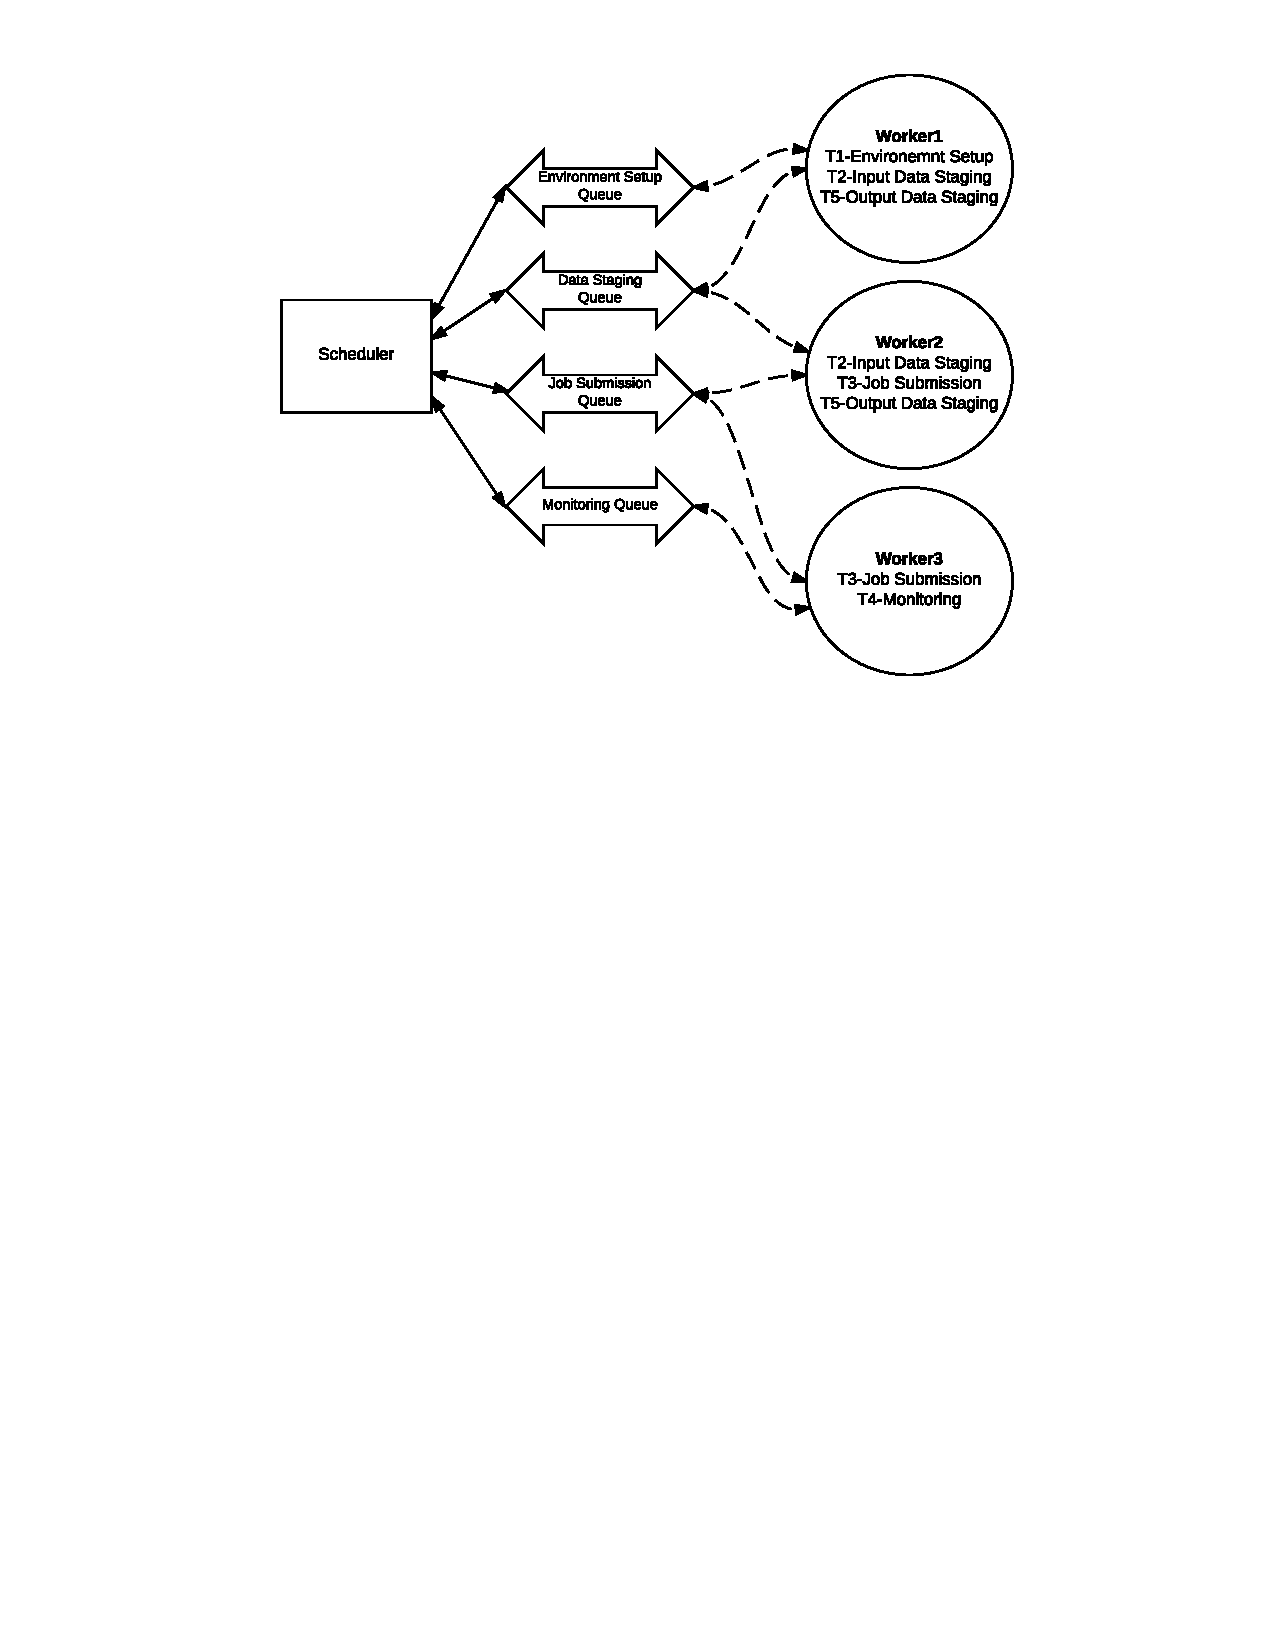
\includegraphics[height=3in, width=3.5in]{figures/scheduler-pull-mechanism.pdf}
\caption{Scheduler-Worker interaction using RabbitMQ messaging queues.}
\end{figure*}

\subsubsection{Push Mechanism - Using Gossip Protocol}
\begin{itemize}
\item A much more intelligent scheduler which constantly receives updates from every worker - using gossip protocol - about the workers existence and capabilities \cite{kermarrec2007gossiping}.
\item Scheduler uses this information to make informed decision about which worker to assign a task to, upon receiving a SchedulingRequest from the Orchestrator.
\item Based on the attributes received from the worker, the scheduler can be configured to use any scheduling algorithm to decide task assignment to a worker.
\end{itemize}

\begin{figure*}
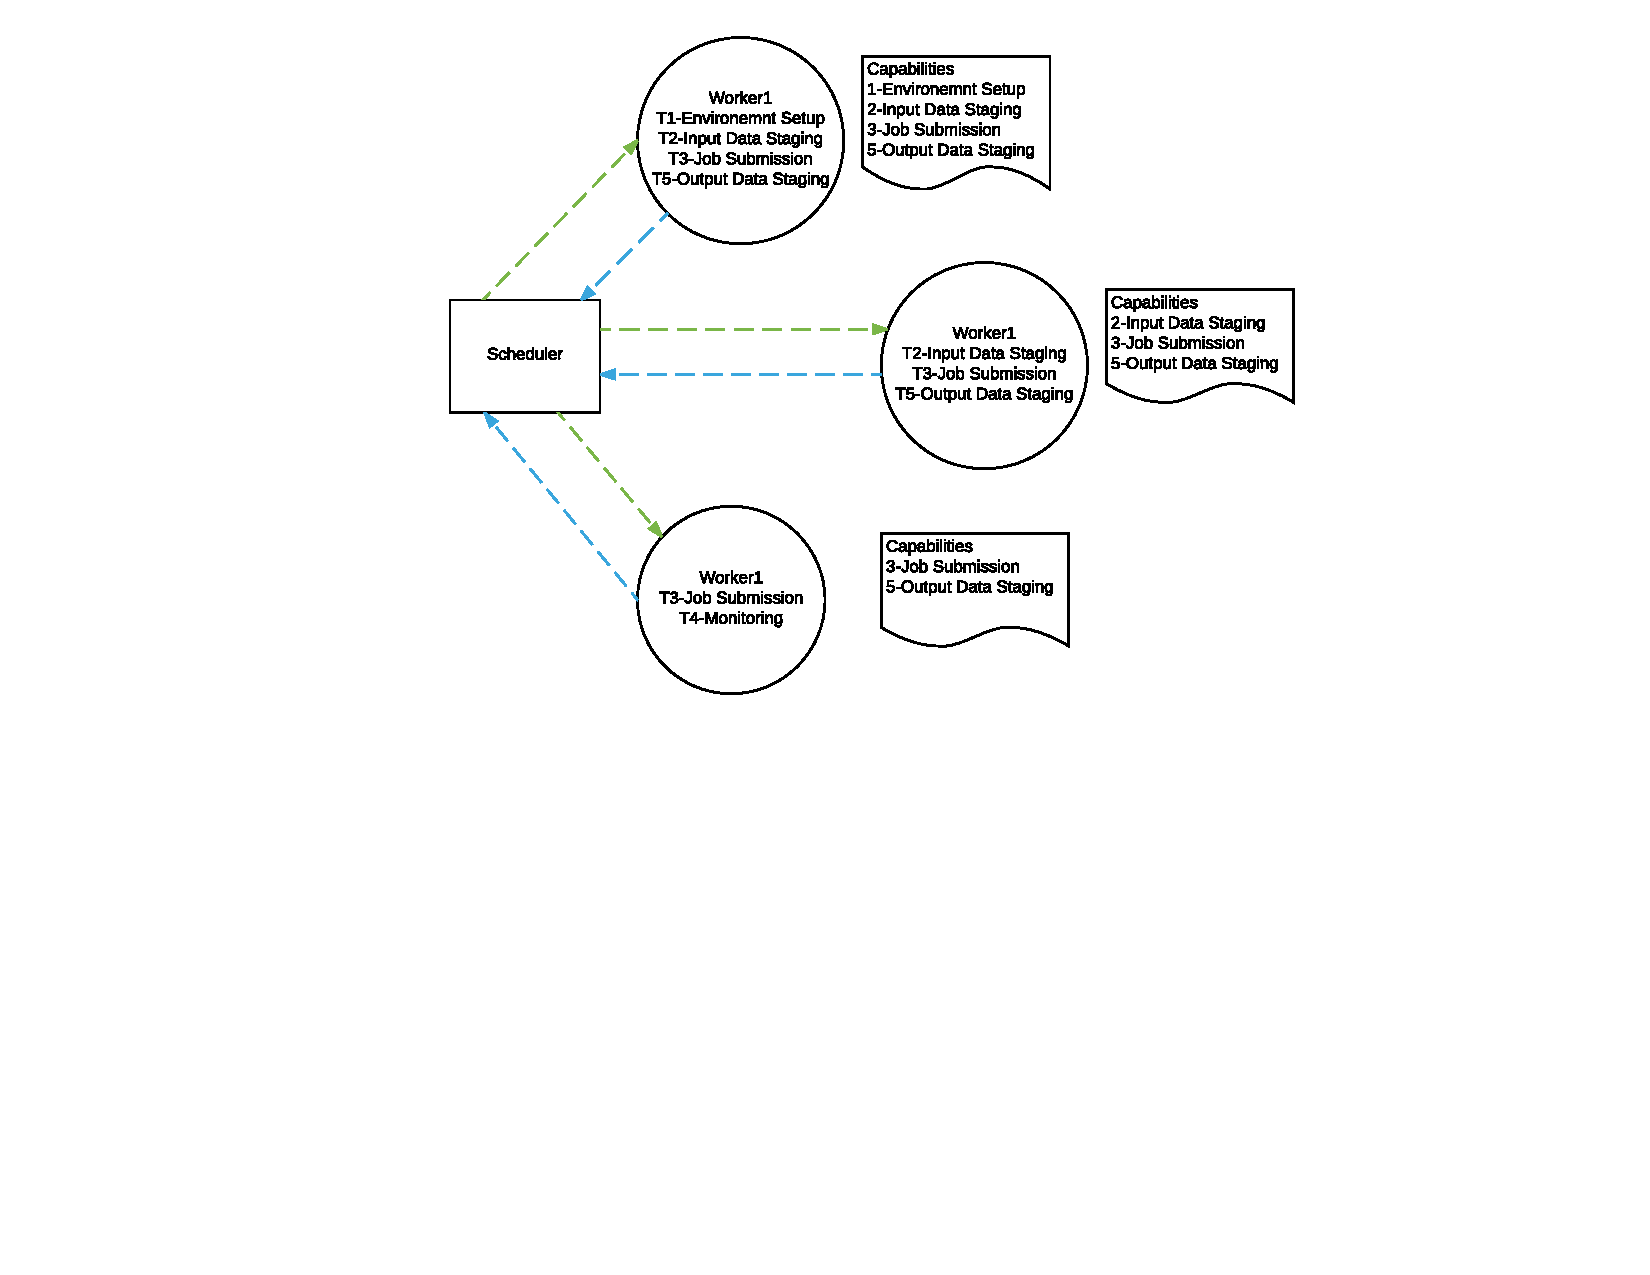
\includegraphics[height=3in, width=3.5in]{figures/scheduler-push-mechanism.pdf}
\caption{Scheduler-Worker interaction using Gossip Protocol}
\end{figure*}

\section{RELATED WORK}

\subsection{Matchmaking using HTCondor}
HTCondor architecture is very similar to our proposed design; it offers a robust workload management system for compute-intensive jobs. It provides a job queueing mechanism, scheduling, priority scheme, monitoring, and resource management. HTCondor employees a matchmaking algorithm to schedule jobs on particular nodes \cite{coleman2001implementation}. It uses ClassAd mechanism for matching resource requests (jobs) with nodes \cite{coleman2003distributed}. Whenever a job is submitted to Condor, it states both the requirements and the preferences, such as required memory, name of the program to run, user who submitted the job, and a rank for the node that will run the job. Also, nodes advertise their capacities in terms of RAM, CPU type and speed, current load with other static and dynamic properties.

Schedulers continuously read all the job ClassAds and all the node ClassAds and ensure that the requirement in both ClassAds are satisfied before scheduling any jobs on a node. HTCondor can be used to build a highly-scalable Grid-style computing environment.  It makes use of cutting edge Grid and cloud-based computing designs and protocols. HTCondor can be used to build Grid-style computing environments that cross administrative boundaries. 

\subsection{AKKA's Actor Model}
AKKA uses an Actor-Director model to provide elegant solutions in a distributed environment. Essentially, this model employees lightweight event-driven processes to provide a robust platform for applications. It raises the abstraction level by hiding low-level non-blocking I/O, concurrency, parallelism and distribution. AKKA provides a strong set of APIs for java and scales to control the lifecycle of the actors.

\section{CONCLUSIONS AND FUTURE WORK}
We have been able to come up with a flexible solution for distributed task execution. Considering its advantages, we are hoping to integrate this design in current Apache Airavata architecture. However, before Airavata code can absorb this framework it needs to go through certain improvements. We are working through the prototype to make these improvements. 

In its current capacity, implemented prototype supports pull mechanism between scheduler and workers. Here, we are depending on messaging infrastructure (RabbitMQ) for delegating tasks to workers. This approach works well, but as we move ahead, systems might need to absorb surprising business demands.  Therefore, we prefer to retain control over task delegation rather than depending on third party technologies. The push mechanism would give better control over workers and task execution. One can think of using a matchmaking algorithm used by HTCondor where workers can advertise their capabilities in terms of task implementation, available memory, current load, CPU speed, etc.  In these situations the scheduler can match task requirements with available workers and assign tasks accordingly. Also, the scheduler can monitor node heartbeats to maintain worker\textquotesingle s states and can spin up new instances as required. Again, one can think of gossip protocol to communicate state and resource information. Serf is a widely used gossip protocol which inherently supports scalability and fault tolerance. 

Also in this prototype we have used RabbitMQ for communication between Orchestrator and Scheduler. Considering it could be a single point of failure one can think of using a more robust, scalable and fault tolerant messaging infrastructure. Kafka is a very good contender, and we are planning to come up with better communication infrastructure which would satisfy the needs of scalability and fault-tolerance, yet give a very good control over message flow.   

%\begin{acks}
%  The authors would like to thank Dr. Yuhua Li for providing the
%  matlab code of  the \textit{BEPS} method. 
%
%  The authors would also like to thank the anonymous referees for
%  their valuable comments and helpful suggestions. The work is
%  supported by the \grantsponsor{GS501100001809}{National Natural
%    Science Foundation of
%    China}{http://dx.doi.org/10.13039/501100001809} under Grant
%  No.:~\grantnum{GS501100001809}{61273304}
%  and~\grantnum[http://www.nnsf.cn/youngscientsts]{GS501100001809}{Young
%    Scientsts' Support Program}.
%
%\end{acks}

\bibliographystyle{ACM-Reference-Format}
\bibliography{distributed-task-execution} 

\end{document}
